\chapter{Reusable Spellbooks: Functions}

\begin{figure}[h!]
    \centering
    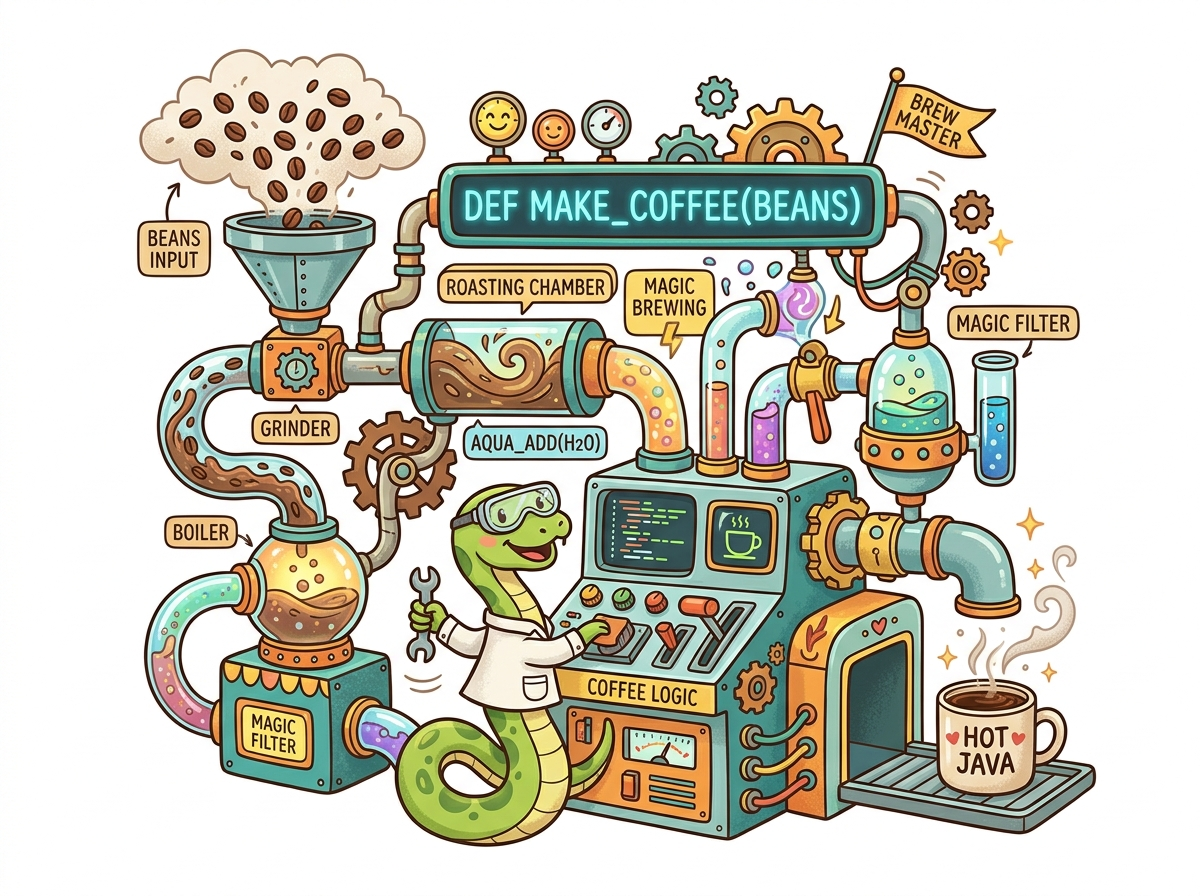
\includegraphics[width=0.75\textwidth]{images/ch4_magic_machine.jpg}
    \caption{Functions are like magic coffee brewing machines: feed them inputs, get delicious results!}
\end{figure}

\section{Don't Repeat Yourself (DRY Principle)}

Copying and pasting the same code 5 times in your program is a crime against humanity. If you find a bug in that code later, you will have to fix it in 5 different places (and you will forget place \#4).

A \textbf{function} is a bundled block of reusable code. You define it once, name it, and call it whenever you need it!

\section{Defining and Calling Functions}

We use the keyword \texttt{def} to define a function, followed by the function name and parentheses \texttt{()}.

\begin{pycode}{Basic Function}
# 1. Defining the magic spell
def cast_fireball():
    print("WHOOSH! A fiery explosion illuminates the room!")

# 2. Calling the spell
cast_fireball()
cast_fireball()
\end{pycode}

\section{Parameters \& Arguments: Feeding the Machine}

Functions become 10x more useful when you feed them input values called \textbf{parameters}.

\begin{pycode}{Functions with Inputs}
def greet_wizard(wizard_name, spell_element="Ice"):
    print(f"Greetings, Archmage {wizard_name}! Master of {spell_element}!")

# Positional arguments
greet_wizard("Gandalf", "Light")

# Using default parameter values
greet_wizard("Merlin")
\end{pycode}

\section{Return Values: Receiving the Loot}

Functions don't just display text; they can calculate a value and hand it back to you using the \texttt{return} keyword.

\begin{pycode}{Returning Values}
def calculate_potion_price(base_cost, tax_rate):
    total = base_cost * (1 + tax_rate)
    return total  # Handing the result back

cost = calculate_potion_price(100, 0.08)
print(f"Total Potion Cost: ${cost:.2f}")
\end{pycode}

\begin{viperpitfall}{Print vs Return}
\texttt{print()} displays text on the screen for human eyes.
\texttt{return} hands data back to the program so other variables can store it!
If your function lacks a \texttt{return} statement, Python implicitly returns \texttt{None}!
\end{viperpitfall}

\section{Scope: What Happens in Functions Stays in Functions}

Variables created inside a function live in a private bubble called \textbf{local scope}. They disappear into thin air the moment the function finishes executing!

\begin{pycode}{Local Scope Demo}
def secret_vault():
    gold_coins = 9999  # Local variable
    print("Inside vault:", gold_coins)

secret_vault()
# Trying print(gold_coins) outside here will crash with NameError!
\end{pycode}

\section{Code Example: Flexible Function Arguments}

Python allows functions to accept flexible arguments using \texttt{*args} (multiple positional inputs) and \texttt{**kwargs} (multiple keyword inputs).

\begin{pycode}{Flexible Function Arguments}
def summon_minions(*minion_names, **details):
    print(f"Summoning {len(minion_names)} minions:")
    for minion in minion_names:
        print(f" - Minion: {minion}")
    
    if "location" in details:
        print(f"Rally Point: {details['location']}")

summon_minions("Bob", "Stuart", "Kevin", location="Dungeon B3")
\end{pycode}

\section{Practice Problems \& Exercises}

Cast your spellbook skills on these 3 function problems!

\begin{snakelab}{Problem 4.1: Tip Calculator Function (Easy)}
Write a function called \texttt{calculate\_tip(bill\_amount, tip\_percentage=15)}.
It should return the calculated tip amount. Test it with a \$50 bill at 15\% and 20\% tip!
\end{snakelab}

\begin{pycode}{Solution 4.1: Tip Calculator}
def calculate_tip(bill_amount, tip_percentage=15):
    return bill_amount * (tip_percentage / 100)

tip1 = calculate_tip(50.00)      # Default 15%
tip2 = calculate_tip(50.00, 20)  # Custom 20%

print(f"15% Tip on $50: ${tip1:.2f}")
print(f"20% Tip on $50: ${tip2:.2f}")
\end{pycode}

\begin{snakelab}{Problem 4.2: Palindrome Detector Function (Medium)}
Write a function called \texttt{is\_palindrome(word)} that returns \texttt{True} if a string reads the same backwards and forwards (ignoring case), and \texttt{False} otherwise.
Test it with \texttt{"Racecar"} and \texttt{"Python"}.
\end{snakelab}

\begin{pycode}{Solution 4.2: Palindrome Detector}
def is_palindrome(word):
    cleaned = word.lower().replace(" ", "")
    return cleaned == cleaned[::-1]

print("Is 'Racecar' a palindrome?", is_palindrome("Racecar"))
print("Is 'Python' a palindrome?", is_palindrome("Python"))
\end{pycode}

\begin{snakelab}{Problem 4.3: Find Max of Three Numbers (Spicy)}
Write a function called \texttt{max\_of\_three(a, b, c)} that returns the largest of three numbers WITHOUT using Python's built-in \texttt{max()} function!
\end{snakelab}

\begin{pycode}{Solution 4.3: Max of Three Numbers}
def max_of_three(a, b, c):
    if a >= b and a >= c:
        return a
    elif b >= a and b >= c:
        return b
    else:
        return c

result = max_of_three(42, 99, 17)
print(f"The maximum among 42, 99, and 17 is: {result}")
\end{pycode}
